% CCIS extended working manuscript, revised 13 November 2026.
% Compile main.tex. Results and x86 wrapping validation remain in progress.
% The original sources are retained in the dated backup directory.
\documentclass[runningheads]{llncs}
\usepackage[T1]{fontenc}
\usepackage{amsmath}
\usepackage{newtxtext}
\usepackage[varvw]{newtxmath}
\usepackage{graphicx}
\usepackage{xcolor}
\usepackage{booktabs}
\usepackage{tabularx}
\usepackage{array}
\usepackage{tikz}
\usetikzlibrary{positioning,arrows.meta}
\usepackage{xurl}
\usepackage[hidelinks]{hyperref}
\urlstyle{same}
\providecommand{\Description}[1]{}
\setlength{\emergencystretch}{2em}
\newcolumntype{Y}{>{\raggedright\arraybackslash}X}
\definecolor{draftblue}{RGB}{24,73,114}
\newif\ifworkingdraft
\workingdrafttrue % Set false only after completing the result tables and notes.
\newcommand{\draftnote}[1]{\ifworkingdraft\par\smallskip\noindent
  {\color{draftblue}\small\textbf{Draft note.} #1}\par\smallskip\fi}
\newcommand{\pending}{\textit{pending}}
\newcommand{\dev}{\textit{in development}}
\begin{document}
\title{Zone: Code--Data Identification and LLM-Assisted Metamorphism for Windows Payloads}
\titlerunning{Code--Data Identification and LLM-Assisted Metamorphism}
\author{Stefano~Bistarelli\orcidID{0000-0001-7411-9678} \and
Jacopo~Di~Benedetto \and
Francesco~Santini\orcidID{0000-0002-3935-4696}}
\authorrunning{S. Bistarelli et al.}
\institute{Dipartimento di Matematica e Informatica, Universit\`a degli Studi di Perugia,\\
Via Vanvitelli 1, 06123 Perugia (PG), Italy\\
\email{stefano.bistarelli@unipg.it}\\
\email{jacopo.dibenedetto@studenti.unipg.it}\\
\email{francesco.santini@unipg.it}}
\maketitle
\begin{abstract}
Binary metamorphism depends on recovering executable instructions while
preserving embedded data and the references that connect them. This article
extends Zone, a binary-to-binary rewriting engine for compact Windows x86
and x64 payloads, with code--data identification and LLM-assisted
transformation. One identification path combines bounded symbolic
exploration, control-flow recovery, and complementary heuristics; another
uses an LLM to propose data ranges for a shared deterministic data-handling
layer. A separate LLM pipeline transforms assembly using four established
transformation families and supports zero-shot and two-shot prompting.
The extension also integrates assembly wrapping, an existing technique,
with an x86 port under development. The assessment distinguishes
classification quality, build success, empirical functionality,
static-scan verdicts, representation similarity, output diversity, and
generation cost. The conference experiments provide a separately
identified historical baseline. This separation permits analysis of
which conclusions follow from classification, validation, and execution
evidence, and which require further investigation.
\keywords{Binary Rewriting \and Code--Data Identification \and
Metamorphic Code \and Large Language Models \and Functional Preservation}
\end{abstract}
\draftnote{Working manuscript: extended experiments are in progress.
New numerical results remain explicitly pending. The x86 wrapping port is
development work, not a validated result. Add the principal verified
findings to this abstract before submission.}
\section{Introduction}\label{sec:introduction}
Rewriting a binary changes the evidence available to an analyst without
necessarily changing the computation that the binary performs. This
distinction motivates the study of metamorphic transformations, both as
a software-protection mechanism and as a challenge for malware
analysis~\cite{PEsurveybible,metamorphic1,metamorphic2}. A useful assessment
must establish what was transformed, whether the intended behavior was
retained, and how the resulting representation was measured. These
questions become particularly difficult when executable instructions and
embedded data share a raw binary address space.

Zone provides a payload-level setting in which to investigate these
questions. Its binary-to-binary interface accepts compact Windows x86
and x64 inputs without source code or debugging information. The original
engine implements instruction substitution, insertion, and control-flow
transformations, including the Position-Independent Instruction (PII)
representation introduced in our SECRYPT 2026
paper~\cite{zone_secrypt_2026}. The present work retains that scope while
expanding the analysis and transformation paths.

\paragraph{Motivation.}
A sequence of bytes can be both a valid instruction encoding and part of
a string or another data object. Successful decoding therefore provides
insufficient evidence that the bytes should be rewritten as instructions.
The conference study identified this ambiguity as a source of functional
failures. Addressing it requires more than a different transformation:
the engine must identify candidate data, preserve its contents, and
maintain the references through subsequent layout changes. Failures at
any of these stages can invalidate an otherwise well-formed output.

LLMs introduce two further questions. They can be used to classify
regions of a binary, and they can be asked to transform an assembly
representation. The first task produces candidate labels or intervals;
the second produces a new instruction sequence. They have different
outputs, validation requirements, and failure modes. We consequently
study them as separate components, even though both interact with the
same data-handling infrastructure.

\paragraph{Relationship to the Conference Paper and Contributions.}
The original engine, PII design, and initial experiments appeared
in~\cite{zone_secrypt_2026}. The present article synthesizes that material
as a historical baseline and adds the following work:
\begin{enumerate}
\item A code--data identification layer combining bounded symbolic
exploration, static control-flow recovery, and complementary heuristics,
with an alternative LLM-based identification path and shared deterministic
data handling.
\item An LLM-assisted assembly-transformation pipeline for four
transformation families, with explicit zero-shot and two-shot conditions,
structural validation, and feedback after rejected attempts.
\item Integration of assembly wrapping, an existing technique, into Zone,
with the x64 implementation distinguished from the x86 port currently
under development.
\item An expanded assessment framework separating identification quality,
construction success, functional outcomes, static-scan observations,
similarity, diversity, and computational cost.
\end{enumerate}
The results of the additional campaigns are kept separate from the
published measurements. Reused visual material is attributed at its
point of use. The statement accompanying the submission details these
differences for the editors.

\paragraph{Scope.}
The subject is raw payload rewriting rather than complete Portable
Executable (PE) transformation. PE sections, imports, relocations, and
loader behavior introduce dependencies outside the experiments considered
here. Payload-level functional checks also capture only the behavior
observed by the chosen harness. Neither a valid assembly listing nor an
accepted raw-file scan establishes preservation of all program behaviors
or the response of a deployed endpoint product.

The article first introduces the relevant work
(Section~\ref{sec:background}) and Zone's architecture
(Section~\ref{sec:architecture}). Sections~\ref{sec:code_data},
\ref{sec:llm}, and~\ref{sec:wrapping} describe the extensions.
Section~\ref{sec:methodology} defines the assessment, and
Section~\ref{sec:results} separates historical and extended results.
Section~\ref{sec:discussion} discusses validity and remaining limitations;
Section~\ref{sec:conclusions} concludes.

\section{Background and Related Work}\label{sec:background}
\subsection{Metamorphism and Binary Rewriting}
Metamorphic transformation changes the program body rather than merely
changing an encoded copy and a decoder. Earlier engines explored
register substitution, instruction replacement, and code reorganization;
their development and detection are discussed
in~\cite{historycodeobf,desai2008towards,desai2010highly,szor2001hunting}.
Surveys place these approaches within the broader space of obfuscation
and malware transformation~\cite{survey1,brezinski2023metamorphic,PEsurveybible}.

Zone uses four established transformation families in addition to PII.
Equal code substitution (EQ) changes the instruction representation of
an operation. NOP insertion adds operations intended to leave relevant
state unchanged. Instruction block permutation (IBP) changes the physical
order of blocks while retaining their logical succession. Bogus control
flow (BCF) adds paths with predetermined outcomes and regions excluded
from the intended execution. These names describe transformation goals;
correctness depends on the treatment of flags, registers, memory, and
control-flow references in each implementation.

Compiler-based obfuscation, exemplified by
Obfuscator-LLVM~\cite{llvmobf}, operates with intermediate representations
and information unavailable to a raw-binary rewriter. Native binary
rewriting must first recover the instructions and references that it
will modify~\cite{bin2binobf}. This difference is central to the
code--data problem examined here.

\subsection{Code--Data Identification}
A disassembler assigns an instruction interpretation to byte sequences;
that interpretation need not reflect the role of the bytes during
execution. Linear decoding can traverse embedded strings, whereas
control-flow recovery can miss paths that depend on unresolved values.
The difficulties of recovering control flow from binaries have been
studied beyond the payload setting~\cite{staticdisasmTuringComplete}.

The angr framework exposes static control-flow recovery and symbolic
execution as distinct forms of analysis~\cite{angr_cfg_docs}. The former
provides candidate blocks; the latter can provide evidence of addresses
visited under a model and resource budget. Missing environmental behavior
and incomplete exploration limit both the recovered graph and the
interpretation of unvisited addresses. The identification layer in this
article combines these sources of evidence with explicit heuristics.
It does not equate an unvisited byte with a proven data byte.

\subsection{LLMs for Assembly Analysis and Transformation}
Prior research has investigated LLM-generated metamorphic variants and
assembly-level obfuscation, including the MetamorphASM study and its
evaluation setting~\cite{llm2,llmobf}. Such work motivates examining model
outputs as structured artifacts that require assembly and validation.
The ability to produce plausible assembly is distinct from preserving
the behavior of a particular input.

Our extension separates two applications. The identification task asks
for candidate data ranges. The transformation task asks for a modified
assembly program under a specified transformation family. Deterministic
checks surround both tasks, so the evaluated object is a complete
pipeline as well as the model's initial proposal. The number of examples
in the first prompt and the presence of subsequent feedback are reported
separately.

\subsection{Assembly Wrapping and Related Representations}
Assembly wrapping exploits the possibility of overlapping instruction
interpretations. The technique and its antecedents are discussed
in~\cite{assembly_wrapping}. We adopt its established name and attribute
the underlying idea; the contribution here is its implementation and
assessment within Zone. It also exposes a measurement issue: a
disassembly obtained from one entry interpretation may differ from the
instruction stream actually followed during execution.

Polymorphic encoding provides a complementary comparison. Shikata Ga Nai
(SGN) combines an encoded body with a variable decoding
routine~\cite{sgnarticle,sgn64,sgnstrong}. The recovered body can be
examined after decoding, a scenario related to attack-code extraction
from memory~\cite{codeExtraction}. This distinction concerns the
representation presented to analysis; it does not imply a general
ranking of endpoint defenses.

Defensive research includes statistical sequence models, behavior-based
identification, and learned signatures for metamorphic
programs~\cite{wong2006hunting,identifyingmeth,methgenetic,metamorphic1}.
Accordingly, the static-scan observations considered in this article
represent one measurement setting among several relevant forms of
analysis.

\section{Zone Architecture}\label{sec:architecture}
\subsection{Input Scope and Instruction Representation}
Zone's payload implementation is written in Python and uses Capstone
for disassembly and Keystone for assembly. The project is publicly
available.\footnote{\url{https://github.com/jakydibe/Zone}.}
Its x64 and x86 paths share the same broad organization but require
architecture-specific handling of operands and references. Support in
one path is therefore not evidence of support in the other.

Instruction objects retain an association with the original decoding
and the current representation. Address-indexed lookup and tracked
control-flow references allow layout updates to be propagated through
the instruction sequence. A rewriting operation can change the size of
an instruction, its address, or the physical relation between blocks;
the final output must reflect the resulting layout rather than the
addresses in the first decoding.

The initial decoding is itself fallible. Decoder options that skip
undecodable bytes allow processing to continue, but do not establish
which successfully decoded bytes are genuine code. Full decoding
coverage is a useful structural check and remains insufficient as a
semantic criterion. The extended data layer addresses a different part
of this problem by retaining explicit candidate data and reference
information.

\subsection{The Published PII Design}\label{sec:pii}
PII was introduced in the conference article~\cite{zone_secrypt_2026}.
It separates logical execution order from the physical placement of
instruction units. The published representation uses wrapped original
operations, a redirector, and an offset table. The table identifies the
next logical unit after the current operation; physical adjacency is
therefore not the sole representation of succession.
Figure~\ref{fig:pii_layout} retains the original layout as architectural
context. It describes the conference design rather than a new method
introduced in this extension.
\begin{figure}[t]
\centering
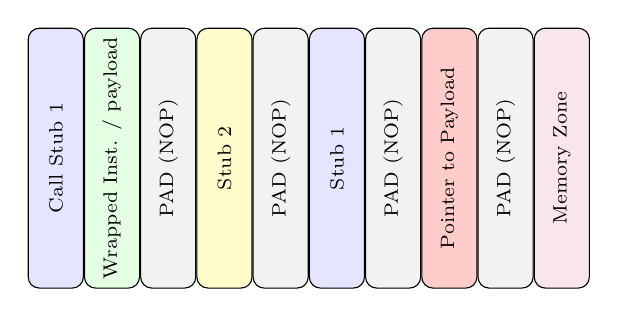
\begin{tikzpicture}[
    font=\scriptsize,
    node distance=0.0cm,
    every node/.style={
        rotate=90,
        minimum width=3.3cm,
        minimum height=0.7cm,
        text centered,
        draw,
        fill=gray!10,
        rounded corners,
        inner xsep=2pt,
        inner ysep=6pt
    }
]

\node (stubCall)  [fill=blue!10]    {Call Stub 1};
\node (payload)   [below=of stubCall, fill=green!10]  {Wrapped Inst. / payload};
\node (pad1)      [below=of payload]                  {PAD (NOP)};
\node (stub2)     [below=of pad1, fill=yellow!20]     {Stub 2};
\node (pad2)      [below=of stub2]                    {PAD (NOP)};
\node (stub1)     [below=of pad2, fill=blue!10]       {Stub 1};
\node (pad3)      [below=of stub1]                    {PAD (NOP)};
\node (payloadPtr)[below=of pad3, fill=red!20]        {Pointer to Payload};
\node (pad4)      [below=of payloadPtr]               {PAD (NOP)};
\node (memZone)   [below=of pad4, fill=purple!10]     {Memory Zone};

\end{tikzpicture}
\Description{A schematic separates the initial call, instruction wrappers, redirector components, padding, offset information, and memory region.}
\caption{PII payload layout. Adapted from Fig.~1 of~\cite{zone_secrypt_2026}.}
\label{fig:pii_layout}
\end{figure}

The state used by dispatch must be preserved independently of the state
used by the original operation. Control-flow instructions and
architecture-specific addressing also require dedicated handling.
The extension distinguishes the original PII design from later
implementation revisions. It also distinguishes a dispatcher-based
representation from single-instruction permutation with explicit
successors. These paths are not interchangeable experimental labels.

\subsection{Extended Architecture}
Figure~\ref{fig:extended_architecture} organizes the added functionality
into identification, deterministic data handling, transformation, and
validation. The identification methods are alternatives. Both supply
candidate regions to the data layer, while the LLM transformation path
uses an assembly representation prepared by the engine. The model is
not responsible for the entire binary-writing infrastructure.

\begin{figure}[t]
\centering
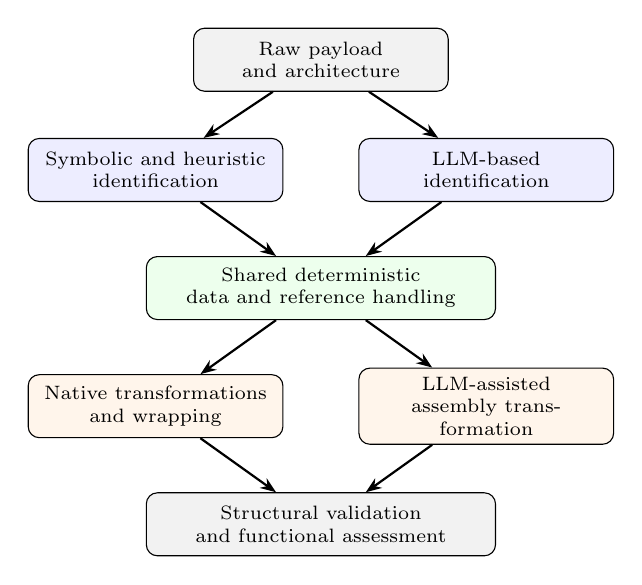
\begin{tikzpicture}[font=\scriptsize,
 box/.style={draw,rounded corners,align=center,minimum height=8mm,text width=30mm},
 arr/.style={-{Stealth[length=2mm]},thick}]
\node[box,fill=gray!10] (input) at (0,0) {Raw payload\\and architecture};
\node[box,fill=blue!7] (sym) at (-2.1,-1.4) {Symbolic and heuristic\\identification};
\node[box,fill=blue!7] (llmdata) at (2.1,-1.4) {LLM-based\\identification};
\node[box,fill=green!7,text width=42mm] (data) at (0,-2.9) {Shared deterministic\\data and reference handling};
\node[box,fill=orange!8] (native) at (-2.1,-4.4) {Native transformations\\and wrapping};
\node[box,fill=orange!8] (llm) at (2.1,-4.4) {LLM-assisted\\assembly transformation};
\node[box,fill=gray!10,text width=42mm] (validation) at (0,-5.9) {Structural validation\\and functional assessment};
\draw[arr] (input)--(sym); \draw[arr] (input)--(llmdata);
\draw[arr] (sym)--(data); \draw[arr] (llmdata)--(data);
\draw[arr] (data)--(native); \draw[arr] (data)--(llm);
\draw[arr] (native)--(validation); \draw[arr] (llm)--(validation);
\end{tikzpicture}
\caption{Conceptual organization of the extended system. Identification
and transformation paths are selected according to the experimental
condition; the diagram does not assert that every combination is supported.}
\label{fig:extended_architecture}
\Description{Two alternative identification paths feed shared data handling,
followed by native or LLM-assisted transformation and validation.}
\end{figure}

The implementation distinguishes original input identity, intermediate
code and data representations, and final output identity. This matters
for both reference handling and measurement. For example, similarity
against a canonicalized intermediate representation measures a different
change from similarity against the original file. Likewise, a data
analysis retrieved from a cache is not a new symbolic exploration.

\begin{table}[t]
\caption{Implementation scope of the extensions in this working draft.
Availability does not imply completed empirical validation.}
\label{tab:scope}
\centering\small
\begin{tabularx}{\linewidth}{@{}Yll@{}}
\toprule
Component & x64 & x86 \\
\midrule
Symbolic/heuristic identification & Implemented & Implemented \\
LLM data identification & Implemented & Implemented \\
LLM EQ/NOP/BCF/IBP & Implemented & Implemented \\
Assembly wrapping & Implemented & \dev \\
Extended quantitative assessment & In progress & In progress \\
\bottomrule
\end{tabularx}
\end{table}

Table~\ref{tab:scope} records the current development boundary.
The support matrix will be finalized against the version used for the
reported campaigns. Ongoing development, especially the x86 wrapping
port, is not merged into an already completed experimental condition.

\section{Code--Data Identification and Data-Preserving Rewriting}
\label{sec:code_data}
\subsection{Problem Definition}
Let an input payload be a byte sequence $B=(b_0,\ldots,b_{n-1})$.
The identification task returns candidate data intervals
$[s_j,e_j)$ in payload-relative coordinates, optionally accompanied by
a kind such as an ASCII string, a UTF-16LE string, or another data object.
A candidate identifies a proposed role for the bytes. Its acceptance
for rewriting additionally depends on the available reference evidence
and the capabilities of the data-handling layer.

This distinction is important for strings stored directly after code.
Some bytes of a string may decode successfully as arithmetic, I/O, or
branch instructions. The conference paper illustrated the problem with
\texttt{calc.exe}. Table~\ref{tab:inline_example} retains a shortened
form of that example to motivate the extension. The presence of a valid
instruction encoding is not a sufficient reason to transform the
corresponding bytes.

\begin{table}[t]
\caption{Selected bytes from the inline-data example in Table~5
of~\cite{zone_secrypt_2026}, reproduced as motivation for code--data
identification.}
\label{tab:inline_example}
\centering\small
\begin{tabular}{@{}lll@{}}
\toprule
Offset & Bytes or characters & Decoder interpretation \\
\midrule
\texttt{0x10b} & \texttt{c} & \texttt{.byte 0x63} \\
\texttt{0x10d} & \texttt{l} & \texttt{insb byte ptr [rdi], dx} \\
\texttt{0x10f} & bytes of \texttt{.exe} & \texttt{js 0x178} \\
\bottomrule
\end{tabular}
\end{table}

The task also includes uncertainty. A region outside the recovered graph
may contain data, unobserved code, or a mixture of the two. The pipeline
retains the origin of a candidate rather than collapsing all such
regions into the same evidential category. This permits separate
assessment of candidate generation, filtering, and downstream outcomes.

\subsection{Symbolic and Heuristic Identification}
The non-LLM path combines static graph information with bounded symbolic
exploration. A CFGFast pass supplies candidate code blocks and inferred
data objects. Symbolic exploration records instruction addresses visited
under the raw-payload model. An additional graph-recovery pass can use
newly observed entries, so that dynamically observed code is not lost
merely because it was absent from the first graph.

The symbolic initial state models uninitialized registers and memory
symbolically. It does not initialize a complete Windows process or
implement all external API behavior. Exploration is bounded by a time
budget, a state/block-step limit, a pending-state limit, and solver
budgets. Reports record the stop reason and unresolved states. Reaching
a resource limit, encountering an unsupported operation, and exhausting
the current frontier have different meanings and are reported
separately.

The implementation maintains evidence at byte granularity by expanding
observed instruction starts into their decoded spans. This avoids
treating the interior bytes of an observed instruction as unexecuted
data candidates. Candidate strings are then identified with printable
ASCII and UTF-16LE patterns, including their terminators. Overlap with
observed code prevents acceptance under this string heuristic.

Static graph recovery can itself classify a string as code. For a
string that overlaps candidate graph code, the implementation requires
additional structural corroboration rather than relying on printability
alone. Other proposed regions originate from graph-inferred data or
from bytes outside recovered blocks. The latter remain uncertain and
are distinguished from stronger data candidates.

The analysis returns intervals, their kinds, and diagnostic information;
it does not prove a complete partition of the payload into code and
data. In particular, a byte not observed during this run is not thereby
proven unreachable or safe to move. The experimental assessment records
both the proposed intervals and the limits of the run that produced them.

\subsection{LLM-Based Identification}
The alternative identification path presents the input through a hex
view, a linear disassembly, and candidate printable runs. These are
different views of the same bytes. The disassembly is explicitly
heuristic, and the printable runs are candidate evidence rather than
reference labels. The model returns structured data ranges, including
offset and length, instead of a rewritten binary.

The parser checks that intervals have positive lengths, remain within
the input bounds, and do not overlap. The engine then associates
candidate ranges with its existing reference information. Ranges that
cannot be accepted by the configured pipeline are reported or rejected.
A fresh engine instance is used when applying a proposal, avoiding
reuse of partially modified state after a rejected answer.

An invalid answer can trigger another request with feedback. The
reported outcome therefore distinguishes the first proposal, later
proposals, and the final accepted result. This distinction is necessary
to attribute an observation correctly: a useful final extraction may
reflect both the model's proposal and deterministic filtering.

The number of worked examples in this classification prompt is recorded
independently of the transformation experiment. A zero-shot/two-shot
comparison of assembly transformation does not imply that the same
comparison has been performed for identification.

\subsection{Shared Data and Reference Handling}
Both identification paths connect to deterministic data-handling
routines. These routines preserve the contents selected for extraction,
track the references whose interpretation depends on the data layout,
and finalize supported references after the code layout is known.
Identification answers which regions are candidates; reference handling
determines which proposed operations are supported by the implementation.

Different architectures require different addressing treatment. The
x64 and x86 implementations therefore share a conceptual contract
without being assumed identical at operand level. A candidate accepted
in one architecture need not be accepted in the other. The evaluation
keeps architecture and reference category associated with the outcome.

The pipeline also checks output integrity, including consistency of
the preserved data contents and the supported references. These checks
can prevent an invalid output from being accepted, but they cannot
establish that all references in an arbitrary binary have been recovered.
An unsupported case is consequently distinguished from a successfully
handled case and from an output that is built but fails execution.

Analysis caching is a practical part of the implementation. Candidate
data can be reused for an input identity, while references are recomputed
against the working representation. Reproducibility requires recording
whether an identification result was computed or retrieved and the
configuration associated with the cached entry. Timing comparisons
separate these cases.

\subsection{Classification Outputs and Residual Uncertainty}
Three outputs are retained for analysis: raw candidate intervals,
intervals accepted by deterministic checks, and intervals ultimately
processed by the data layer. Equal final binaries do not establish
equal raw classifications, because filtering can remove differences.
Conversely, a correct candidate can be rejected because its reference
pattern is unsupported. That rejection is an integration limitation,
not necessarily a classification error.

The evaluation in Section~\ref{sec:methodology} therefore separates
classification quality from downstream functionality. Successful
execution supplies evidence about the observed behavior after data
handling, while reference annotations supply evidence about the byte
roles. Neither observation can substitute for the other.

\section{LLM-Assisted Assembly Transformation}\label{sec:llm}
\subsection{Task and Supported Transformation Families}
The transformation path asks an LLM to produce a complete modified
assembly representation for a selected family: EQ, NOP insertion, BCF,
or IBP. These families retain their meanings from the native engine;
the use of a model changes how the proposed representation is produced.
Each request selects one family so that the generated artifact and its
validation policy have an identifiable experimental condition.

PII and assembly wrapping remain native paths in the version examined
here. They are not described as LLM-generated techniques. Likewise, a
native condition combining transformations is not automatically
equivalent to several model calls in sequence. The experiment identifies
the implemented path rather than grouping all uses of the same family
under one label.

\subsection{Assembly Representation and Data Boundary}
The engine prepares an assembly representation with symbolic labels
for the relevant locations and preserves the data representation
outside the model-generated instruction text. This preparation defines
an intermediate input to the transformation task. It also determines
the reference point for several structural checks and similarity
measurements.

The model's text is assembled and associated with the data retained by
the engine. The output is therefore a product of model generation,
assembly, data handling, and validation. The experimental record retains
the identity of the original file, the intermediate representation,
and the final bytes, so that preparation-induced changes can be
distinguished from changes in the model's output.

\subsection{Zero-Shot and Two-Shot Conditions}
The initial zero-shot request contains the task specification without
worked examples. The initial two-shot request contains two examples
in addition to that specification. The example identities and prompt
versions are part of the experimental condition. Differences in their
content, not only their number, can influence the comparison.

These labels apply to the first request in a run. After rejection, a
later request may contain the previous answer and validation feedback.
Such a run remains assigned to its initial prompting condition, but its
later attempts are explicitly feedback-assisted. Reporting only the
final accepted output would hide this additional interaction.

The experimental unit is a run under a specified input, transformation,
prompt condition, and generation configuration. Repeated run numbers
are not claimed to be independently controlled model seeds unless the
service accepts and records such a parameter. Temperature, token
budget, model identifier, and service configuration are recorded
separately from the run index.

\subsection{Validation and Feedback}
Validation covers several kinds of structural evidence. Assembly must
succeed, the produced code must meet the decoding checks, tracked branch
destinations must have appropriate boundaries, and the expected data
representation must remain consistent. Additional checks depend on the
selected family and examine whether the output still contains the
required instruction structure or applies a nontrivial transformation.

These checks are deliberately narrower than semantic equivalence.
An output can pass structural validation yet behave differently; a
conservative check can also reject an output that would have performed
the expected behavior. The assessment records the reason for each
rejection rather than treating all rejected answers as one category.

For supported test cases, a functional verifier can participate in the
generation loop. If that verifier is also used to select accepted
outputs, a later test based on the same observable is conditional on
selection. The article distinguishes this pipeline acceptance criterion
from an independent functional assessment and reports attempts that
exhaust the allowed budget.

\subsection{What Is Attributed to the Model}
Three aspects are considered separately: whether an answer can be
assembled, whether the complete pipeline accepts it, and whether an
accepted output satisfies the reported functional check. Deterministic
preparation and validation are part of the system contribution rather
than capabilities attributed to the model alone.

The run record includes elapsed time, API usage when supplied by the
service, rejected attempts, and the accepted artifact. Estimated cost
is derived from the stated tariff snapshot; it is not presented as an
invoice. Resumed jobs and reused outputs are identified so that they
are not counted as additional generation calls.

\section{Integration of Assembly Wrapping}\label{sec:wrapping}
\subsection{Existing Technique and Contribution}
Assembly wrapping is an established technique based on alternative
instruction interpretations~\cite{assembly_wrapping}. Its inclusion in
this article does not claim invention of the underlying idea. The
extension contributes an implementation in Zone, interaction with the
engine's instruction and data representations, and a separate empirical
assessment.

The relevant conceptual property is that the instruction interpretation
obtained by a particular static decoding need not be the instruction
stream followed during execution. This property makes it especially
important to identify which representation is used by a similarity or
coverage measurement. A statistic from the static view and one from
the intended execution view answer different questions.

\subsection{Integration and Supported Inputs}
Wrapping is integrated with the native rewriting infrastructure and
depends on an instruction representation adequate for the selected
input. It must also interact with the final data layout and the
references affected by changes in instruction placement. Construction
can be refused when the required input interpretation is incomplete
or an unsupported case is encountered.

Some instructions or local regions are handled differently from the
main wrapped representation. The assessment therefore records the
proportion represented by wrapping, retained regions, output size,
construction failures, and functional outcomes. A claim about the
whole output must not be inferred solely from the fraction of
instructions accepted by one internal stage.

The experiment distinguishes wrapping alone, the chosen combined
native condition, and the corresponding preparation-only controls.
Their names identify complete configurations, including data handling
and architecture. Implementation availability and successful build
are reported separately from empirical functionality.

\subsection{x86 Port and Development Status}
The x64 implementation is available for assessment. The x86 port is
under active development at the time of this draft. Register width,
instruction encodings, and addressing assumptions require
architecture-specific treatment, so an x64 outcome is not transferred
to the x86 column of a result table.

The result layout reserves separate x86 entries. Those entries remain
marked as development work until a frozen version and its assessment
are available. If the port changes during a campaign, its new results
are associated with the new version; they are not silently appended
to results from an earlier implementation.

\subsection{Assessment Boundary}
Wrapping is assessed with the same separation of construction,
functionality, and representation measurements used for other methods.
In particular, a failure to construct an output remains part of the
overall outcome. Reporting functionality only for constructed binaries
can describe accepted artifacts but does not describe availability
across all attempted cases. Section~\ref{sec:methodology} defines both
denominators.

\section{Experimental Methodology}\label{sec:methodology}
\subsection{Research Questions and Experimental Units}
The extended assessment addresses four questions:
\begin{description}
\item[RQ1:] How do the symbolic/heuristic and LLM identification paths
compare in candidate quality, agreement, coverage, and analysis cost?
\item[RQ2:] What construction and functional outcomes are observed
after data handling and transformation, and which failure stages
account for unsuccessful cases?
\item[RQ3:] What are the observed outcomes and representation changes
for assembly wrapping in each assessed architecture?
\item[RQ4:] How do zero-shot and two-shot LLM transformation differ
in initial and final acceptance, functional outcomes, similarity,
diversity, time, and cost?
\end{description}

The input payload is the unit for comparisons across methods. A run
identifies one input and one configuration, while an attempt is a
generation or validation step within that run. Multiple variants of
one payload are repeated observations of the same input rather than
independent samples of the Windows software population. Scan engines
and repeated submissions of identical bytes are also not treated as
independent payloads.

\subsection{Corpora, Versions, and Configuration Matrix}
The conference corpus consists of 102 inputs, divided into 38 x64 and
64 x86 payloads~\cite{zone_secrypt_2026}. Extended campaigns are described
by their own manifests. A subset selected for poor historical outcomes
is identified as such; its aggregate result is not presented as a new
measurement on all 102 inputs.

Table~\ref{tab:campaign_manifest} reserves the information needed to
reconstruct each campaign. Distinct payload count, repeated runs,
constructed files, and unique output hashes remain separate counts.
The final record includes input hashes, engine version or snapshot
hash, architecture, prompt version, model configuration, and dependency
versions. For identification, the analysis limits and cache status are
also recorded.

\begin{table}[t]
\caption{Extended campaign manifest. Pending entries await the frozen
experimental datasets; the historical corpus is specified in the text.}
\label{tab:campaign_manifest}
\centering\small
\begin{tabularx}{\linewidth}{@{}Ylll@{}}
\toprule
Campaign & Inputs & Architectures & Replicates \\
\midrule
Code--data identification & \pending & x64/x86 & \pending \\
Data handling and native methods & \pending & x64/x86 & \pending \\
Assembly wrapping & \pending & x64 & \pending \\
Assembly wrapping port & \pending & x86 (development) & \pending \\
LLM transformation, 0/2 shot & \pending & \pending & \pending \\
\bottomrule
\end{tabularx}
\end{table}

Model aliases can change independently of the client. The identifier
sent in a request, the version returned by the service when available,
and any version label assigned locally are therefore distinguished.
A locally maintained tariff or alias table is not independent
confirmation of the model version used by the provider.

\subsection{Identification Quality and Reference Annotations}
Where reference annotations are available, data is treated as the
positive class. Let $G$ be the set of annotated data-byte offsets and
$P$ the set predicted by the method. The byte-level measures are
\begin{align}
\mathrm{Precision}_{D} &= \frac{|P\cap G|}{|P|}, &
\mathrm{Recall}_{D} &= \frac{|P\cap G|}{|G|},\\
F_{1,D} &= \frac{2\,\mathrm{Precision}_{D}\,\mathrm{Recall}_{D}}
 {\mathrm{Precision}_{D}+\mathrm{Recall}_{D}}.
\end{align}
Undefined cases, including inputs without reference data, are reported
explicitly rather than assigned a favorable score. Code bytes predicted
as data are counted as false positives and examined separately because
their treatment can invalidate execution.

Interval-level assessment complements byte-level scores. An exact
boundary match and partial overlap are distinguished; the chosen
overlap rule is stated with the results. Any reference bytes left
unresolved by annotation are excluded from binary classification
scores and their coverage is reported. The same treatment is used
for all methods.

Reference labels must be established independently of the evaluated
method and associated with the original input offsets. The assessment
retains raw candidates and post-filtering results separately. It can
therefore attribute an error to identification or to acceptance and
integration, rather than assigning every final outcome to the model.

If independent labels are unavailable, the comparison is reported as
agreement and a case study. Pairwise agreement between two methods,
or byte identity of their final outputs, does not establish accuracy.
Functionality after extraction is likewise reported as a downstream
check rather than used to construct reference labels.

\subsection{Build Success and Functional Outcomes}
Let $N$ be the number of planned cases, $B$ the number producing an
accepted binary, and $W$ the number passing the stated functional check.
The assessment reports
\begin{equation}
\mathrm{BuildRate}=B/N,\qquad
\mathrm{WorkingRate}_{\mathrm{all}}=W/N,\qquad
\mathrm{WorkingRate}_{\mathrm{built}}=W/B.
\end{equation}
All three counts accompany the percentages. An unbuilt case is not
removed from the first two denominators. An incomplete or unexecuted
case remains distinguishable from a completed failing test.

The functional oracle is specified by payload class. An observed
connection, an opened port, a dialog, and exception-free termination
are different observables with different evidential strength. The
harness version, architecture, observation window, and relevant
configuration are recorded. Original inputs are checked under the
same current harness to characterize its baseline behavior.

These observations do not prove complete semantic equivalence. A
connection can occur before later execution fails; clean termination
may not exercise the intended operation; and a dialog verifies only
the behavior observed by that test. Conclusions retain the scope of
the oracle actually used.

For LLM runs, the record additionally distinguishes initial acceptance,
acceptance within the retry budget, and the outcome of each functional
check. If execution is part of generation-time acceptance, a subsequent
pass rate on selected outputs is labeled accordingly. Exhausted runs
remain in the run-level denominator.

\subsection{Static-Scan Measurements}
For completed file $i$, let $m_i$ be the number of malicious verdicts
and $a_i$ the number of engines included by the stated eligibility rule.
The per-file malicious-verdict fraction and its macro average are
\begin{equation}
d_i=m_i/a_i,\qquad
\overline d=\frac{1}{F}\sum_{i=1}^{F}d_i.
\end{equation}
The file-level detected fraction is a separate measure,
\begin{equation}
q=\frac{1}{F}\sum_{i=1}^{F}\mathbf{1}[m_i>0].
\end{equation}
The term detection rate is not used to interchange these quantities.
The report specifies whether unsupported engines, failed analyses,
and timeouts enter $a_i$, and provides their counts. A pending
analysis has no measured verdict fraction and is not recorded as zero.

Files are submitted or retrieved by content identity. Repeated outputs
with one hash can reuse a scan, while that hash can still belong to
several experimental conditions. Deduplication of scanning is separated
from membership in result groups. The analysis states whether summaries
weight unique binaries, generation runs, or payloads equally.

Scan dates and service metadata are retained. Historical and current
campaigns may use different engine versions and submission contexts.
Differences across such campaigns are not attributed solely to the
transformation. Raw-binary verdicts are interpreted within their file
format and service setting, without extrapolation to deployed endpoint
detection.

\subsection{Similarity, Diversity, and Representation Size}
Every similarity score specifies its representation and reference.
The sequence-based validation score in the current LLM path uses
normalized instruction signatures and the matching-block ratio exposed
by \texttt{SequenceMatcher}~\cite{python_difflib}. If $M$ signature
elements occur in the selected matching blocks and the sequence lengths
are $u$ and $v$, the ratio is $2M/(u+v)$. This is not cosine similarity.

Normalization removes selected literal differences. In the NOP
condition the implementation also removes recognized no-op operations
before comparison. A score of one after that filtering indicates
agreement under the defined representation; it does not indicate
byte-identical files. The exact normalization version is retained with
the experiment.

For frequency-based comparison, let $A$ and $B$ be nonzero vectors
under a common token vocabulary. Cosine similarity is
\begin{equation}
\mathrm{CosSim}(A,B)=\frac{A\cdot B}{\|A\|\,\|B\|}.
\end{equation}
The report states whether tokens are mnemonics alone or include
operands, and whether the vectors describe an original/output pair
or pooled corpus text. These constructions are not combined in one
unqualified similarity column. With wrapping, the decoding view used
to obtain tokens is also stated.

Output diversity is measured independently of similarity to an input.
The basic exact measure reports distinct hashes among completed
outputs, both within a condition and across conditions. Repeated
generation does not imply distinct bytes. Size is recorded as bytes
and, for matched pairs, as $(L_{\mathrm{out}}-L_{\mathrm{in}})/L_{\mathrm{in}}$.
Any entropy statistic identifies whether its symbols are raw bytes or
assembly tokens; it remains descriptive rather than evidence of
functional preservation.

\subsection{Time, Cost, and Aggregation}
The timing record separates analysis, preparation, model calls, local
validation, and the stated total where these are available. Cached
analysis and reused outputs are distinguished from newly computed
runs. Costs include failed generation attempts as well as final
accepted artifacts. Their currency, tariff date, and estimation rule
are specified.

Results are stratified by architecture and input population before
aggregation. Repeated variants of the same input remain grouped when
estimating uncertainty. For small pilots, individual counts and
distributions are reported and broad population-level claims are
avoided. Any statistical comparison is accompanied by its unit of
analysis, uncertainty method, and treatment of missing observations.
\draftnote{Finalize the campaign manifests, reference annotations,
harness configuration, scan eligibility rule, model settings, and
aggregation policy from the frozen experiment records.}

\section{Experimental Results}\label{sec:results}
\subsection{Published Experimental Baseline}\label{sec:baseline}
The conference experiments provide historical context for the
extensions~\cite{zone_secrypt_2026}. Their corpus contained 102 Windows
payloads: 38 x64 and 64 x86. Fifteen single and combined transformation
configurations were considered, with ten variants planned for each
input/configuration pair. Planned multiplicity is distinguished from
the number of outputs actually available.

Table~\ref{tab:historical} summarizes selected published aggregate
observations. The original-file malicious-verdict means were 21.67\%
for x64 and 22.63\% for x86. The published transformed-file averages were
substantially smaller, but functional outcomes varied across
configurations. These measurements belong to the original engine,
corpus, harness, and scan periods. They are not new experiments on the
extensions described above.

\begin{table}[t]
\caption{Selected published aggregate static-scan observations,
summarized from~\cite{zone_secrypt_2026}. Percentages describe the
published malicious-verdict fractions, not deployed endpoint detection.}
\label{tab:historical}
\centering\small
\begin{tabular}{@{}lrr@{}}
\toprule
Published condition & x64 & x86 \\
\midrule
Original payloads & 21.67\% & 22.63\% \\
Zone configurations, reported average & 0.57\% & 0.25\% \\
SGN comparison & 0.00\% & 10.22\% \\
\bottomrule
\end{tabular}
\end{table}

The conference comparison with SGN also considered memory dumps after
decoding~\cite{zone_secrypt_2026}. Such a submission tests recognition
of recovered bytes, whereas Zone's intended model retains a rewritten
representation. Neither observation directly measures the runtime
response of an installed endpoint product. The comparison is retained
as historical context rather than evidence about the new LLM or
wrapping paths.

The historical figures for size, entropy, and similarity characterized
representation changes. Their metrics remain distinct from functional
checks. The extended assessment uses the explicit definitions in
Section~\ref{sec:methodology}; any reanalysis of historical artifacts
must state its own grouping, deduplication, and representation choices.
\draftnote{The previous draft's detailed historical plots are omitted
pending reconciliation of category/value mappings and metric provenance.
The original sources are preserved in the backup. Finalize actual
historical output counts and identify any corrected reanalysis explicitly.}

\subsection{Code--Data Identification}\label{sec:data_results}
\draftnote{Insert the frozen identification campaign here. If no
independent reference annotations are available, present agreement and
case studies and retain that scope in the abstract and conclusions.}
\begin{table}[t]
\caption{Identification assessment. A dash denotes an unavailable
reference-based measure; pending denotes an experiment not yet finalized.}
\label{tab:data_results}
\centering\small
\begin{tabularx}{\linewidth}{@{}Yllll@{}}
\toprule
Method and output stage & Inputs & Precision$_D$ & Recall$_D$ & $F_{1,D}$ \\
\midrule
Symbolic/heuristic candidates & \pending & \pending & \pending & \pending \\
Symbolic/heuristic accepted & \pending & \pending & \pending & \pending \\
LLM candidates & \pending & \pending & \pending & \pending \\
LLM accepted & \pending & \pending & \pending & \pending \\
\bottomrule
\end{tabularx}
\end{table}
The completed analysis will distinguish interval agreement, uncertainty,
filtering, and downstream behavior. Examples will identify whether a
disagreement originates in the proposed data ranges, reference support,
or subsequent transformation. Identical final binaries will be reported
as pipeline agreement rather than used as a substitute for reference
annotations.

\subsection{Functional Assessment of the Extended Engine}
\label{sec:functional_results}
\draftnote{Insert preparation-only and native-transformation outcomes,
with the input-selection rule, architecture, snapshot, and harness.
Keep historical and current MessageBox oracles distinct.}
\begin{table}[t]
\caption{Functional assessment structure. Report counts before
percentages; $N$, $B$, and $W$ are defined in the methodology.}
\label{tab:functional_results}
\centering\small
\begin{tabularx}{\linewidth}{@{}Ylllll@{}}
\toprule
Condition & Arch. & $N$ & $B$ & $W/N$ & $W/B$ \\
\midrule
Data handling only & x64 & \pending & \pending & \pending & \pending \\
Data handling only & x86 & \pending & \pending & \pending & \pending \\
Native transformations & x64 & \pending & \pending & \pending & \pending \\
Native transformations & x86 & \pending & \pending & \pending & \pending \\
\bottomrule
\end{tabularx}
\end{table}
The failure analysis will distinguish construction refusal, incomplete
decoding, unsupported references, failed execution checks, and
uncompleted tests. Aggregate improvement will be interpreted alongside
changes in dependencies, implementation, and the observation protocol.

\subsection{Assembly Wrapping}\label{sec:wrapping_results}
\draftnote{Complete x64 outcomes from the frozen wrapping campaign.
Populate x86 rows only after its development version and evaluation are
fixed. Retain all planned cases, including unsuccessful builds.}
\begin{table}[t]
\caption{Wrapping assessment by architecture and configuration.
The x86 port remains development work in this draft.}
\label{tab:wrapping_results}
\centering\small
\begin{tabularx}{\linewidth}{@{}Yllll@{}}
\toprule
Condition & $N$ & $B/N$ & $W/N$ & $W/B$ \\
\midrule
x64 wrapping & \pending & \pending & \pending & \pending \\
x64 wrapping, combined & \pending & \pending & \pending & \pending \\
x86 wrapping & \multicolumn{4}{c}{\dev} \\
x86 wrapping, combined & \multicolumn{4}{c}{\dev} \\
\bottomrule
\end{tabularx}
\end{table}
The representation assessment will additionally report size, retained
regions, and unique output hashes. Any similarity score will identify
the decoding view. A result restricted to constructed outputs will be
accompanied by construction availability over all planned cases.

\subsection{LLM Transformation: Zero-Shot versus Two-Shot}
\label{sec:llm_results}
\draftnote{Insert the completed 0/2-shot campaign, preserving failed
and repeated runs. Report the number of distinct input payloads and
state whether functional verification participated in selection.}
\begin{table}[t]
\caption{LLM transformation outcomes. Initial and final acceptance
refer respectively to the first attempt and the full retry budget.}
\label{tab:llm_results}
\centering\small
\begin{tabularx}{\linewidth}{@{}Yllll@{}}
\toprule
Family / shots & Runs & Initial acc. & Final acc. & Functional \\
\midrule
EQ / 0 & \pending & \pending & \pending & \pending \\
EQ / 2 & \pending & \pending & \pending & \pending \\
NOP / 0 & \pending & \pending & \pending & \pending \\
NOP / 2 & \pending & \pending & \pending & \pending \\
BCF / 0 & \pending & \pending & \pending & \pending \\
BCF / 2 & \pending & \pending & \pending & \pending \\
IBP / 0 & \pending & \pending & \pending & \pending \\
IBP / 2 & \pending & \pending & \pending & \pending \\
\bottomrule
\end{tabularx}
\end{table}
The comparison will pair those outcomes with attempt counts,
sequence-based similarity, output uniqueness, elapsed time, and cost.
A smaller similarity value will not be interpreted as better functional
preservation, and acceptance after feedback will not be described as
success of the first zero-shot or two-shot answer.

\subsection{Static-Scan and Representation Measurements}
\draftnote{Insert completed scan records and matched representation
measurements. Pending scans are missing observations, never zero
detections. Keep the two verdict measures in distinct columns.}
\begin{table}[t]
\caption{Static-scan reporting structure. Completed hashes and group
membership are distinguished; $\overline d$ and $q$ have different definitions.}
\label{tab:scan_results}
\centering\small
\begin{tabularx}{\linewidth}{@{}Yllll@{}}
\toprule
Group & Unique hashes & Completed & $\overline d$ & $q$ \\
\midrule
Current original controls & \pending & \pending & \pending & \pending \\
Wrapping, by architecture & \pending & \pending & \pending & \pending \\
LLM transformation, by condition & \pending & \pending & \pending & \pending \\
LLM data handling, by condition & \pending & \pending & \pending & \pending \\
\bottomrule
\end{tabularx}
\end{table}
The final discussion will relate these observations to build and
functional outcomes on the same identified artifacts. Static verdicts
for a selected set of constructed binaries will not be generalized
to inputs for which construction or execution failed.

\section{Discussion and Threats to Validity}\label{sec:discussion}
\subsection{Identification and Integration Failures}
Code--data identification and data-preserving rewriting expose related
but distinct failure modes. An incorrect candidate can mark code as
data. A correct candidate may have an unsupported reference. A
successfully processed region may still be followed by an incorrect
transformation elsewhere in the payload. The interpretation of a
working-rate change therefore depends on the stage-level evidence.

Bounded symbolic exploration adds a specific uncertainty: an observed
address establishes that the analysis visited that address under its
model, while absence from the observation set establishes much less.
External Windows behavior, unresolved states, and analysis limits can
leave code unvisited. The heuristic combination and its diagnostics
must remain visible when interpreting the result.

For the LLM path, agreement with another method can characterize shared
outputs without resolving shared errors. Deterministic filtering can
also make different raw answers converge. Reporting candidate and
accepted stages separately is consequently necessary for attribution.

\subsection{Validation, Selection, and Measurement Bias}
Static checks can reject malformed or inconsistent outputs without
proving the behavior of accepted ones. Functional checks narrow the
uncertainty only to the observables exercised by the harness. A
single successful action does not characterize every execution path
or future interaction of a payload.

When the same functional check is part of generation-time selection
and later reporting, the resulting pass rate concerns selected
outputs. It must be read alongside first-attempt acceptance, exhausted
runs, and the complete retry budget. Repeating a failed run until the
campaign contains an accepted artifact changes the selection process
and is retained in the record rather than hidden by the final file.

Similarity introduces another source of interpretation bias. Sequence
matching under normalization, frequency-vector cosine similarity, and
byte identity quantify different relationships. Pooling programs into
one frequency vector also changes the unit of comparison. These
statistics are not interchangeable measures of semantic preservation.
Wrapping further requires the decoding interpretation to be stated.

\subsection{Generalizability and Temporal Validity}
The historical corpus is an identifiable collection of compact
payloads, not a representative sample of all Windows programs. Its
x64 and x86 subsets differ in composition as well as size. A campaign
selected because of earlier failures concentrates on a particular
part of that corpus. Small LLM pilots on one or a few inputs support
case-level observations and require additional evidence for broad
conclusions.

Static-scan services change over time. Engine availability, format
support, and signatures may differ between a historical submission
and a current scan. Even contemporaneous raw-file scans do not
reproduce full application delivery, loading, or endpoint execution.
Observed verdict fractions are therefore interpreted as properties
of the submission setting and the identified artifacts.

Development status is another boundary. The x86 wrapping port is
tracked separately until assessed with a fixed implementation.
Modifying the port during testing can be useful engineering work,
but a combined table must preserve which version produced each row.

\subsection{Defensive Interpretation and Reproducibility}
Binary representation is one source of evidence available to defensive
analysis. Program behavior, memory activity, and repeated toolchain
artifacts can remain informative after a transformation. The
published SGN analyses illustrate recognition opportunities associated
with a common transformation mechanism~\cite{sgnstrong}. Low raw-file
malicious-verdict fractions do not establish absence of those other
signals.

Reproducibility depends on both code and experimental records. The
final artifacts should identify the engine snapshot, input and output
hashes, architecture, dependency versions, prompt examples, complete
attempt accounting, functional oracle, and scan timestamps. Model
aliases and estimated tariffs are time-sensitive metadata. A frozen
record makes the boundaries of an observation inspectable even if
the provider or implementation later changes.
\draftnote{After finalizing the results, replace prospective discussion
with findings supported by the completed tables. Retain the validity
limits that apply to the final protocol.}

\section{Conclusions}\label{sec:conclusions}
The extended Zone architecture makes code--data identification an
explicit component of payload rewriting. Its symbolic and heuristic
path and its LLM-based alternative feed a shared deterministic
data-handling layer. This separation supports analysis of candidate
quality, reference handling, and downstream functionality as distinct
questions.

The transformation extension introduces a separate use of LLMs,
with zero-shot and two-shot conditions and explicit validation and
feedback. Assembly wrapping adds an implementation of an established
technique, while the x86 port remains development work until its
architecture-specific assessment is completed. These contributions
extend the conference design beyond its original transformation
catalogue and experimental baseline.

The assessment framework distinguishes construction, empirical
functionality, static verdicts, similarity, diversity, and cost.
Its purpose is to connect each conclusion to the evidence that can
support it. The historical measurements characterize the earlier
engine and corpus; completed extension results will characterize
the new paths under their stated configurations. Broader claims
about semantic equivalence, unseen inputs, or deployed endpoint
products require evidence outside those boundaries.
\draftnote{Before submission, add the principal verified findings and
the answers to RQ1--RQ4. Update this section and the abstract together;
remove development claims only when the corresponding assessment is
complete.}

\begin{credits}
\subsubsection{\ackname}
This work was partially funded by the University of Perugia's project
``Fighting Cybercrime with OSINT'' (FICO), Civil Safety and Security for
Society (WP2).
\subsubsection{\discintname}
\emph{To be completed by the authors before submission.}
\end{credits}
\bibliographystyle{splncs04}
\bibliography{bibliography}
\end{document}
